
\documentclass[conference]{IEEEtran}
\IEEEoverridecommandlockouts
% The preceding line is only needed to identify funding in the first footnote. If that is unneeded, please comment it out.

%%%%%%%%%%%%%%%%%%%%%%%%%%%%%%%%%%%%%%%%%%%%%%%%%%%%%%%%%%%%%%%%%%%%%%%%%%%%%%%%%%%%%%%%%%%%%%%%%%%%%%%%%%%%
\usepackage{cite}
\usepackage{amsmath,amssymb,amsfonts}
\usepackage{algorithmic}
\usepackage{graphicx}
\usepackage{textcomp}
\usepackage{xcolor}
\def\BibTeX{{\rm B\kern-.05em{\sc i\kern-.025em b}\kern-.08em
    T\kern-.1667em\lower.7ex\hbox{E}\kern-.125emX}}
\makeatletter
\newcommand{\linebreakand}{%
  \end{@IEEEauthorhalign}
  \hfill\mbox{}\par
  \mbox{}\hfill\begin{@IEEEauthorhalign}
}
\makeatother

%%%%%%%%%%%%%%%%%%%%%%%%%%%%%%%%%%%%%%%%%%%%%%%%%%%%%%%%%%%%%%%%%%%%%%%%%%%%%%%%%%%%%%%%%%%%%%%%%%%%%%%%%%%%
\begin{document}

\title{Node-RED based Pet Care IoT Platform \\ using MQTT Messaging Broker
}

\author{
\IEEEauthorblockN{Haeram Kim}
\IEEEauthorblockA{
\textit{Computer Science and Engineering} \\
\textit{Chungnam National University}\\
Daejeon, Korea \\
haeram.kim1@gmail.com
}
\and
\IEEEauthorblockN{Hyejong Kang}
\IEEEauthorblockA{\textit{Computer Science and Engineering} \\
\textit{Chungnam National University}\\
Daejeon, Korea \\
kanghyejong1001@gmail.com}
\and
\IEEEauthorblockN{Sunghan Kim}
\IEEEauthorblockA{\textit{Computer Science and Engineering} \\
\textit{Chungnam National University}\\
Daejeon, Korea \\
seonghan.kim.cnu@gmail.com}
\linebreakand
\IEEEauthorblockN{Dukho Choi}
\IEEEauthorblockA{\textit{International trade / software convergence} \\
\textit{Chungnam National University}\\
Daejeon, Korea \\
dukho.fin@gmail.com}
\and
\IEEEauthorblockN{Jihyun You}
\IEEEauthorblockA{\textit{Computer and Information Technology} \\
\textit{Purdue University}\\
West Lafayette, IN, USA \\
you62@purdue.edu}

}

\maketitle 

%%%%%%%%%%%%%%%%%%%%%%%%%%%%%%%%%%%%%%%%%%%%%%%%%%%%%%%%%%%%%%%%%%%%%%%%%%%%%%%%%%%%%%%%%%%%%%%%%%%%%%%%%%%%%%%%%%%%%%%%
\begin{abstract}
While there are an increasing number of households owning pets, it is challenging for owners who leaves home often to take good care of them. ‘Petification’ can be a solution for pet owners to know if pet is doing well by collecting data from sensors mounted on devices used by pets. Pet’s specific information like daily water intake and the amount of feed a pet eats a day by a visual graph on dashboard. Petification provides status of feed machine and water supplier, such as device connectivity, error existence and the amount of feed or water remaining in the device. When the user wants or when the scheduled time approaches, the feed machine checks the error status and provides feed to the pet if there is no problem. In previous study, mobile application which provides specific datum about pet is already created by using Blynk, but petification implemented a web-based pet IoT platform using Node-RED. MQTT also plays a major role in the data flow as a messaging protocol. In the database, messages are stored over time, and user information, device information, daily statistical information, events to be detected and information on rules, and information on the feeding schedule designated by the user are stored.
\end{abstract}
\hfill\break
\begin{IEEEkeywords}
IoT platform, Node-RED, MQTT, Smart pet care service 
\end{IEEEkeywords}
%%%%%%%%%%%%%%%%%%%%%%%%%%%%%%%%%%%%%%%%%%%%%%%%%%%%%%%%%%%%%%%%%%%%%%%%%%%%%%%%%%%%%%%%%%%%%%%%%%%%%%%%%%%%%%%%%%%%%%%%
\section{Introduction}
The pet care industry is a promising field. Profits from the pet industry increase every year, more than double profit during 10 years, from \$48.4 billion in 2010 to \$109.6 billion in 2020 [1?M.  Hanson.  “Pet  Industry  Statistics”  spots.com.  https://spots.com/pet-industry-statistics/ (accessed Jan. 25, 2022).]. This is because the number of families owning pets is steadily increasing. Figure 1 shows that households owning a dog consists the largest portion, and the number of families owning dogs has increased from 46.3 million in 2011 to 69 million in 2021.

\begin{figure}[htbp]
\centerline{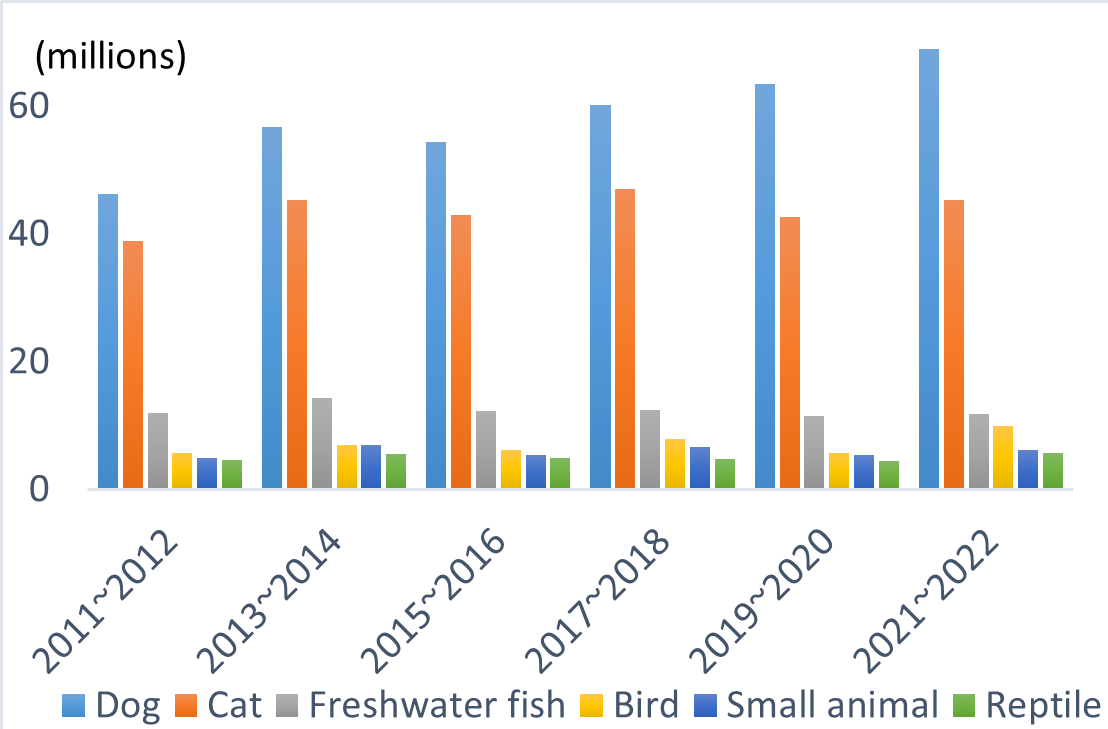
\includegraphics{fig 1.png}}
\caption{Number of U.S. Households That Own a Pet, by Type of Animal
}
\label{fig}
\end{figure}


 As the number of families raising pets increases, the number of pet owners with concerns is increasing. the pet owners' concerns is this. They have to work during the daytime, but there is no way to know their pet is doing well during the day at home.
A way to solve this problem is to receive data remotely about pets in the house at work. Specifically, Internet of Things (IoT) solution may be a solution to this problem.
IoT is a global infrastructure for the information society. IoT enables advanced services by interconnecting interoperable information and communication technologies [?].
Previous researches on pet care IoT has continued like [3?][4?][5?]. Petcare IoT businesses already are operating in market. Pet care IoT Businesses divided into the various field are operating such as health/activity monitor (FitBark [6?], PitPat [7?]), GPS tag(Pawscout [8?], Whistle [9?]),
pet monitor and interactive camera(Petcube [10?]), \textit{et al}. In these businesses, the problem raised above was solved using IoT.

 Our paper focuses on the pet care service part among many IoT solutions. The name of the pet care IoT solution which we implement is 'Petification'. The name petification was created by combining the words pet and notification.
 
 The petification is our overall IoT solution. It provides various information to the owner about whether the pet is doing well while the owner is not at home. Structurally, It is divided into device and software part.   
\subsection{Hardware}
The devices are largely divided into two types: a feed machine and a water supplier. And only feed machine is divided into a bowl part and a container part. Load cell sensors are installed under each part. So totally three load cell sensors were used. The reason for measuring the weight of the feed bowl and the feed container separately is that the weight of the bowl is required to know the feed intake, and the weight of the container is required to know the remaining amount of feed. The devices specific design is like fig 2. The servomotor is attached only to the feed container to control the amount of feed supplied. The edge device delivers data to the platform using a Raspberry pi zero.

\subsection{Software}
When developers implement IoT services, platforms play an important role. The IoT platform is located in the middle of IoT solution, facilitating connection between multiple devices, and connecting platform users and devices. In other words, IoT platforms play a key role in building IoT ecosystems. Because of the importance of IoT platform, we were thinking for a long time about which IoT platform to use. Eventually, Node-red is chosen because we implemented a web-based IoT platform. 

In the entire petification IoT solution, MQTT message broker also plays an important role. The MQTT message broker was used for efficient many-to-many communication and manages the overall data flow in the platform. The MQTT is a protocol that sends messages using publishing and subscribing methods.
Petification's database is MySQL, and most of the data that MQTT messages send and receive by brokers is stored in MySQL.
Pet information data like how much food and water the pet consumed during the day are performed specific logic in the rule engine and then displayed as a graph on the Node-red dashboard.
\\

Chapter 2 (LITERATURE REVIEW) explains previous studies related to pet care which existed before this study. 
Chapter 3 (BACKGROUND) provides the information needed to read this paper.
Chapter 4 (METHODOLOGY) will introduce how we implement the IoT platform.
In Chapter 5  IMPLEMENTATION
Chapter 6 EXPERIMENT
Chapter 7 (CONCLUSION) 
Chapter 8 (ACKNOWLEDGE)

\section{Related Literature}
In this chapter, We will divide the previous studies into device and software aspects. And then previous studies are compared with petification's devices and softwares.

\subsection{Hardware}
[10] Automated Pet Feeder using IoT (IEEE, 2021) In this study, Arduino Uno R3 and SG90 servo motor was used. Distance from the entrance of the feed container to the inside of the bowl is measured using an ultrasonic distance sensor.
However, the petification feed machine used load cell sensors to direct measurement of bowl and container weight. Because we thought that it is difficult to use ultrasonic waves to measure the amount of feed accurately. And the petification feed machine uses Raspberry pi zero and uses MG90S micro servo motor for opening and closing feed gate. 

 [11] Robot Chow: Automatic Animal Feeding with Intelligent Interface to Monitor Pets (IJAERS, 2019) used Raspberry Pi 3. Rotary Valve and DC motor were used to provide feed. The petification feed machine does nots use a rotary valve but uses a gate that can block the feeder container outlet.
 If a rotary valve is used, the amount of feed to be provided to the pet should be determined based on the serving unit contained in one space. On the other hand, the petification feed supply method was selected as the gate method because it has the advantage of being able to adjust the amount of feed to be supplied in more detail than the rotary valve method. In addition, the preceding study of [11] uses a DC motor that is fast, continuous and freely rotatable because feed is supplied through continuous rotation of the rotary valve, but the feed machine of petification use a servo motor because they need more precise control than free continuous rotation.[?] 



\subsection{Software}
  The previous study[?] provides users with food and water consumption, number of defecation and defecation duration using buttons on the app. It was developed through Arduino IDE and was provided with numbers and visual statistics as feed and water consumption, number of defecation and duration real-time using Blynk as an IoT platform.

Previous studies[?] conducted research to implement a system that automatically feeds according to scheduled time and visualizes consumption in real time using Blynk as an IoT platform.


The above two studies commonly used Blynk to implement an IoT platform.
However, Node-RED was used for several reasons in our study instead of Blynk.
1. Visual programming is possible by using nodes. This is a huge advantage because it reduces the development time incredibly. 2. Only the Blynk app can be used for notification in Blynk development environment.
Whereas many other messenger apps are available by using Node-RED. 3. Node-Red is an open source and There are already customized node that can be shared.\hfill\break
\indent For these reasons, petification is implemented using Node-red, which is a major difference from previous studies.
A notification is sent about a malfunction, the consumption of feed and water intake and the feed and water remaining in the container. Then these data are showed in visual graph.
\section{Background}
 \subsection{Used Devices}
Devices commonly used in feed machine and water supplier are 5kg load cell sensors, weight sensor amplifiers(hx711), and Raspberry pi zeros.
The load cell sensor serves to convert the weight or force acting into an electrical signal. [?] 
Hx711 converts an analog signal into a digital signal, amplifies a measured value of a low load cell, and then transmits the value to another microcontroller. [?]
The converted and amplified data in hx711 is transmitted to the Raspberry pi. And then Raspberry pi receives this value and performs calibration.
\hfill \break
\indent Unlike water supplier, servo motor is used in feed machine. The reason why servo motor is used is that, unlike water, feed has to be controlled by opening and closing the gate. A servo motor was used as an actuator to open and close the gate. The servo motor is a rotary or linear actuator that rotates and pushes a machine. [?]


\subsection{Node-RED}
 
 Node-RED is a flow-based development tool that is easy for developers and non-developers to use using visual programming, used to connect hardware devices, APIs, and online services [11?]. It is especially effective when it needs to be visualized quickly like API. Node-RED has operational strengths that it can run in various environments in local, Raspberry Pi, Docker, Cloud Instance, and \textit{et al}. Node-red is an open-source and is being distributed through NPM, so you can utilize nodes or flows created by the user. It also has the advantage of being free and allowing users to customize nodes themselves. User interface (UI) can be configured using Node-RED's node-red-dashboard, and user-friendly UI can be conveniently configured through design changes using CSS and Javascript [12?]. In addition to the node-red-dashboard, many flows can configure the UI, and it is also possible to configure the UI using a third-party library such as React.js. Also Node-RED has the advantage of allowing users to directly access the database and manipulate data, and there are various modules that can be used to send notifications to users. Node-RED is made by International Business Machines Corporation (IBM), and IBM plans to increase its contributor base as an open source for the sustainability of Node-RED. To raise the contributor base, IBM is planning to improve its easy-to-use testing framework, analyze code, and develop Linter, which generates recommendations, warnings, and errors based on what it finds, \textit{et al} [13?].

\subsection{MQTT}
MQTT stands for Message Queuing Telemetry Transport and is the oldest Machine to Machine (M2M) protocol for IoT. It is an ISO standard Publishing-Subscribing-based messaging protocol designed for lightweight M2M communication in a limited network. All MQTT messages have their own topics, and MQTT clients can send and receive data by posting messages to MQTT brokers or subscribing to topics for those messages. TCP is used as a transport protocol, and TLS/SSL can be used for security. This means connection-oriented between Client-Brokers. In the MQTT protocol, three levels of quality of service (QoS) are used, and there are QoS0(), QoS1(), and QoS2(). The MQTT protocol has a small message size and message overhead. In addition, due to low power consumption and resource consumption, it is evaluated as a suitable protocol for use in the IoT field.
[?]

\subsubsection{MQTT vs Other Protocols(CoAP, AMQP, HTTP)}
\hfill \break
In order to select the MQTT protocol, comparative analysis was performed with other protocols.

\paragraph{MQTT vs CoAP}\hfill \break
CoAP uses UDP as a transport protocol, while MQTT uses TCP. The advantage of TCP-based protocols is that they guarantee packet delivery. On the other hand, UDP does not guarantee packet delivery. CoAP is also part of the WEB architecture. It is most suitable for devices that support UDP or UDP analog, but is limited to several special types of IoT devices. On the other hand, MQTT deals with all cases within IoT.[?] 

\paragraph{MQTT vs AMQP}
\hfill \break
AMQP has higher reliability, security, provisioning, and interoperability than MQTT. For this reason, the size and overhead of the message are larger than that of MQTT.
In addition, the amount of power and the use of resources are very large. On the other hand, in the case of the MQTT protocol, the running device consumes little power.
Moreover, due to low overhead, MQTT is often used even in embedded environments for inter-machine communication. An example of using MQTT is a smart home.[?]
\paragraph{MQTT vs HTTP}
\hfill \break
HTTP has the maximum overhead and message size because it is designed for WEB, not IoT. This results in significant latency in Dataflow.
Furthermore, it was judged that the protocol in the IoT platform was inappropriate because the amount of power and resources used was larger than that of MQTT.[?]
Therefore, the MQTT protocol was judged to be suitable for the project in configuring message brokers. The message broker uses Mosquito, which implements the MQTT protocol.

\subsection{Mosquitto}
Mosquito is an open source message broker implementing MQTT protocol versions 5.0, 3.1.1 and 3.1 and is provided by Eclipse. It is also lightweight and suitable for use in all devices, from low-power single board computers to full servers.[?]

There are several programs implementing MQTT, such as EMQ, HiveMQ, Mosquito, and VerneMQ. A study comparing each of the programs suggested that in situations where availability is not significant, using Single Broker and Persistence Setting is a simpler way to configure Message Broker than using clustered Broker [?]. In addition, in the context of using Persistence Setting in Single Broker, Mosquitto had a close 0 percent probability of message loss and message order mixing, and the probability of receiving duplicate messages was significantly lower than that of other programs[?]. Thus, this research uses Mosquitto with persistency setting as single message broker.

\subsection{MySQL}
MySQL is a very fast, flexible, and easy-to-use database with RDBMS (relational database management system). The combination of MySQL's secure processing and reliable software provides effective transactions for large projects, so it is flexible with open sources. MySQL is also excellent in terms of data security because it is evaluated as having the safest and most reliable database management system [?]. In addition, MySQL is considered a suitable database to manage effective data flows because it also has good compatibility with Node-RED [?]. 

\section{Methodology}
The methodology part will be explained by dividing it into the block used for petification and the message flow. The IoT solution of petification is largely divided into three parts: device, platform, and user. This research is conducted with a focus on the development of device and platform. The main blocks used in each of the three parts will be described first and a flowchart will be explained.

\subsection{Blocks}
The platform for this research consists of 8 blocks: MQTT Message Broker and Database are running on independent process, while MQTT Manager, Rule Engine, Device Manager, User Manager, Schedule Engine and UI Dashboard Manager are running on the Node-RED. As a pet-care IoT solution, 2 Devices are attached to the platform: Food Feeder and Water Dispenser. User of the solution can access dashboard which provides pet’s data in a visual way, and they can receives malfunction alert by E-Mail and WhatsApp. Figure 2 shows the overall structure for the proposed pet-care IoT solution.
\begin{figure}[htbp]

\centerline{\includegraphics[width=0.5\textwidth]{platform overall flow.png}}
\caption{Petification overall Structure.}
\label{fig}
\end{figure}

Figure 2 shows the structure and relationship of the pet care platform blocks, devices, and user interface.
\subsubsection{MQTT Message Broker}
\hfill \break This research was conducted with MQTT Protocol to control the message flow. Thus, Mosquitto v1.4.15 was installed and running on the platform server to act as a MQTT Message Broker. Food Feeder, Water Dispenser and Node-RED are connected to the MQTT Message Broker as client, and MQTT Message Broker mediates Node-RED to Device communication and reverse-way communication (Device to Node-RED).

\subsubsection{Database}
\hfill \break To store data efficiently and safely, Database block is included to the platform. As a Database block, MySQL v5.7.37 is installed and running on the platform server. Database stores various data, such as all the MQTT messages (in a Time-series Data Table), message-based action execution rules (in a Rule Table), information for the connected devices (in a Device Table), user information (in a User Table), time-based action execution rules (in a Schedule Table), and daily statistic information (in a Statistic Table).

\subsubsection{MQTT Manager}
\hfill \break MQTT Manager in the Node-RED is the gateway for MQTT messages to enter Node-RED. Main purpose for this block is converting incoming MQTT messages to give convenience to other Node-RED based blocks. To achieve it, this block receives all the messages by subscribing all the MQTT message topic. And then it parses message topic and payload to provide useful information such as username of MQTT session and client id. These informations are used in other Node-RED based nodes in further progress.

\subsubsection{Rule Engine}
\hfill \break The purpose for Rule Engine is activating actions according to MQTT messages. It cooperates with Rule Table of Database to activate action. When one message is published, Rule Engine searches Rule Table to figure out which actions should be activated and activates them. Actions are defined as ReST API form, thus activating action will be progressed as sending a HTTP request. It also provides ReST APIs for adding, modifying and deleting rules. Some ReST APIs for actions are defined in another block, whereas some APIs are defined in Rule Engine, such as updating consumption and sending notifications.

\subsubsection{Device Manager}
\hfill \break Handling devices that are attached by users is the main purpose for Device Manager block. It provides ReST APIs that can add new device to platform (with HTTP POST method), modify status of the device (with HTTP PATCH method) and delete a device (with HTTP DELETE method).

\subsubsection{User Manager}
\hfill \break The purpose for User Manager block is to provide modifying user setting. User can manage these 4 settings: Notification, Email address, WhatsApp information and timezone where user lives. The reason for requiring timezone is to support multi-country users. As managing schedule is done with platform, all the schedules are stored in Database with UTC. Thus timezone for user is needed to convert user’s schedule. All the settings above will be provided with ReST API form.

\subsubsection{Schedule Engine}
\hfill \break Handling and executing schedule is the main functionality for this block. As for schedule execution, it cooperates with Schedule Table in Database. Every minute Schedule Engine checks the Schedule Table and executes the actions that are scheduled to be activated at that time. Also, this block provides ReST APIs that can create, read, update and delete the schedule.

\subsubsection{UI Dashboard Manager}
\hfill \break Dashboard Manager is to provide Graphical User Interface (GUI) to the user. By using this block, user can be provided status of water and food remaining and consumption in a visual way. It also provides buttons to serve food and input areas to set user settings.


\subsection{Flow chart}
% 이 프로젝트의 주요 기능 3가지에 대한 플로우를 설명한다. 느낌
\subsubsection{Flow 1}
\begin{figure}[htbp]
\centerline{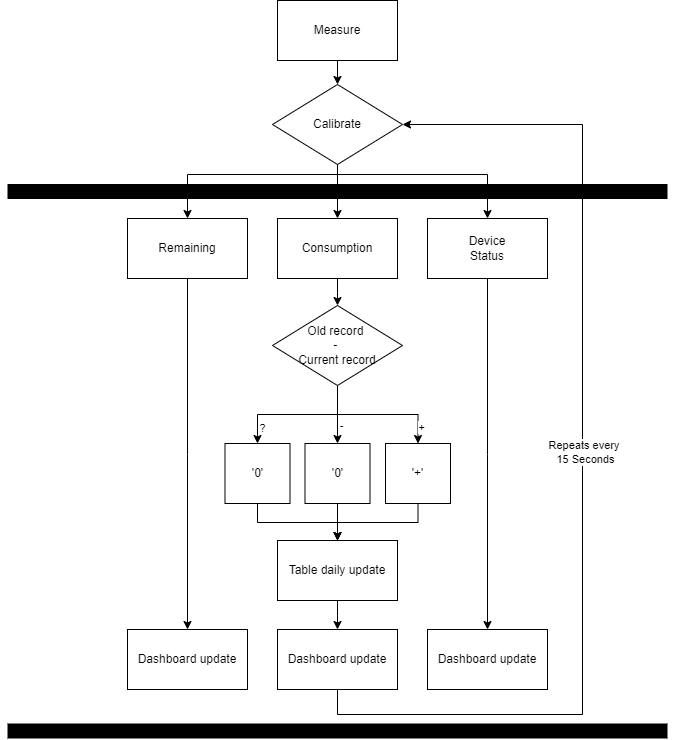
\includegraphics[width=0.5\textwidth]{FlowChart_1.png}}
\caption{Petification flow chart 1.}
\label{fig}
\end{figure}
The load cell sensor measures the value first, and converts the measured value into weight. After that, the three flows proceed in parallel. The first is : updating the remaining feed, the second is : updating the feed intake and the third is : updating the device status.
The remaining feed and device status are immediately displayed on the dashboard, and the feed intake is deducted from the feed amount recorded in the past. If the result is positive, this means that the past record is larger, meaning that the pet consumed feed.
If the resulting value is negative or 0, it means that the current record is larger, meaning that the pet did not consume feed. Therefore, the resulting value comes to zero. In other cases, it is treated as '?'. For example, It is impossible to calculate when there is no previous result value or only the current result value exists. In these three cases described above, data is updated on the table every day and displayed on the dashboard. This overall flow is repeated every 15 seconds.

\hfill \break
\subsubsection{Flow 2}
\begin{figure}[htbp]
\centerline{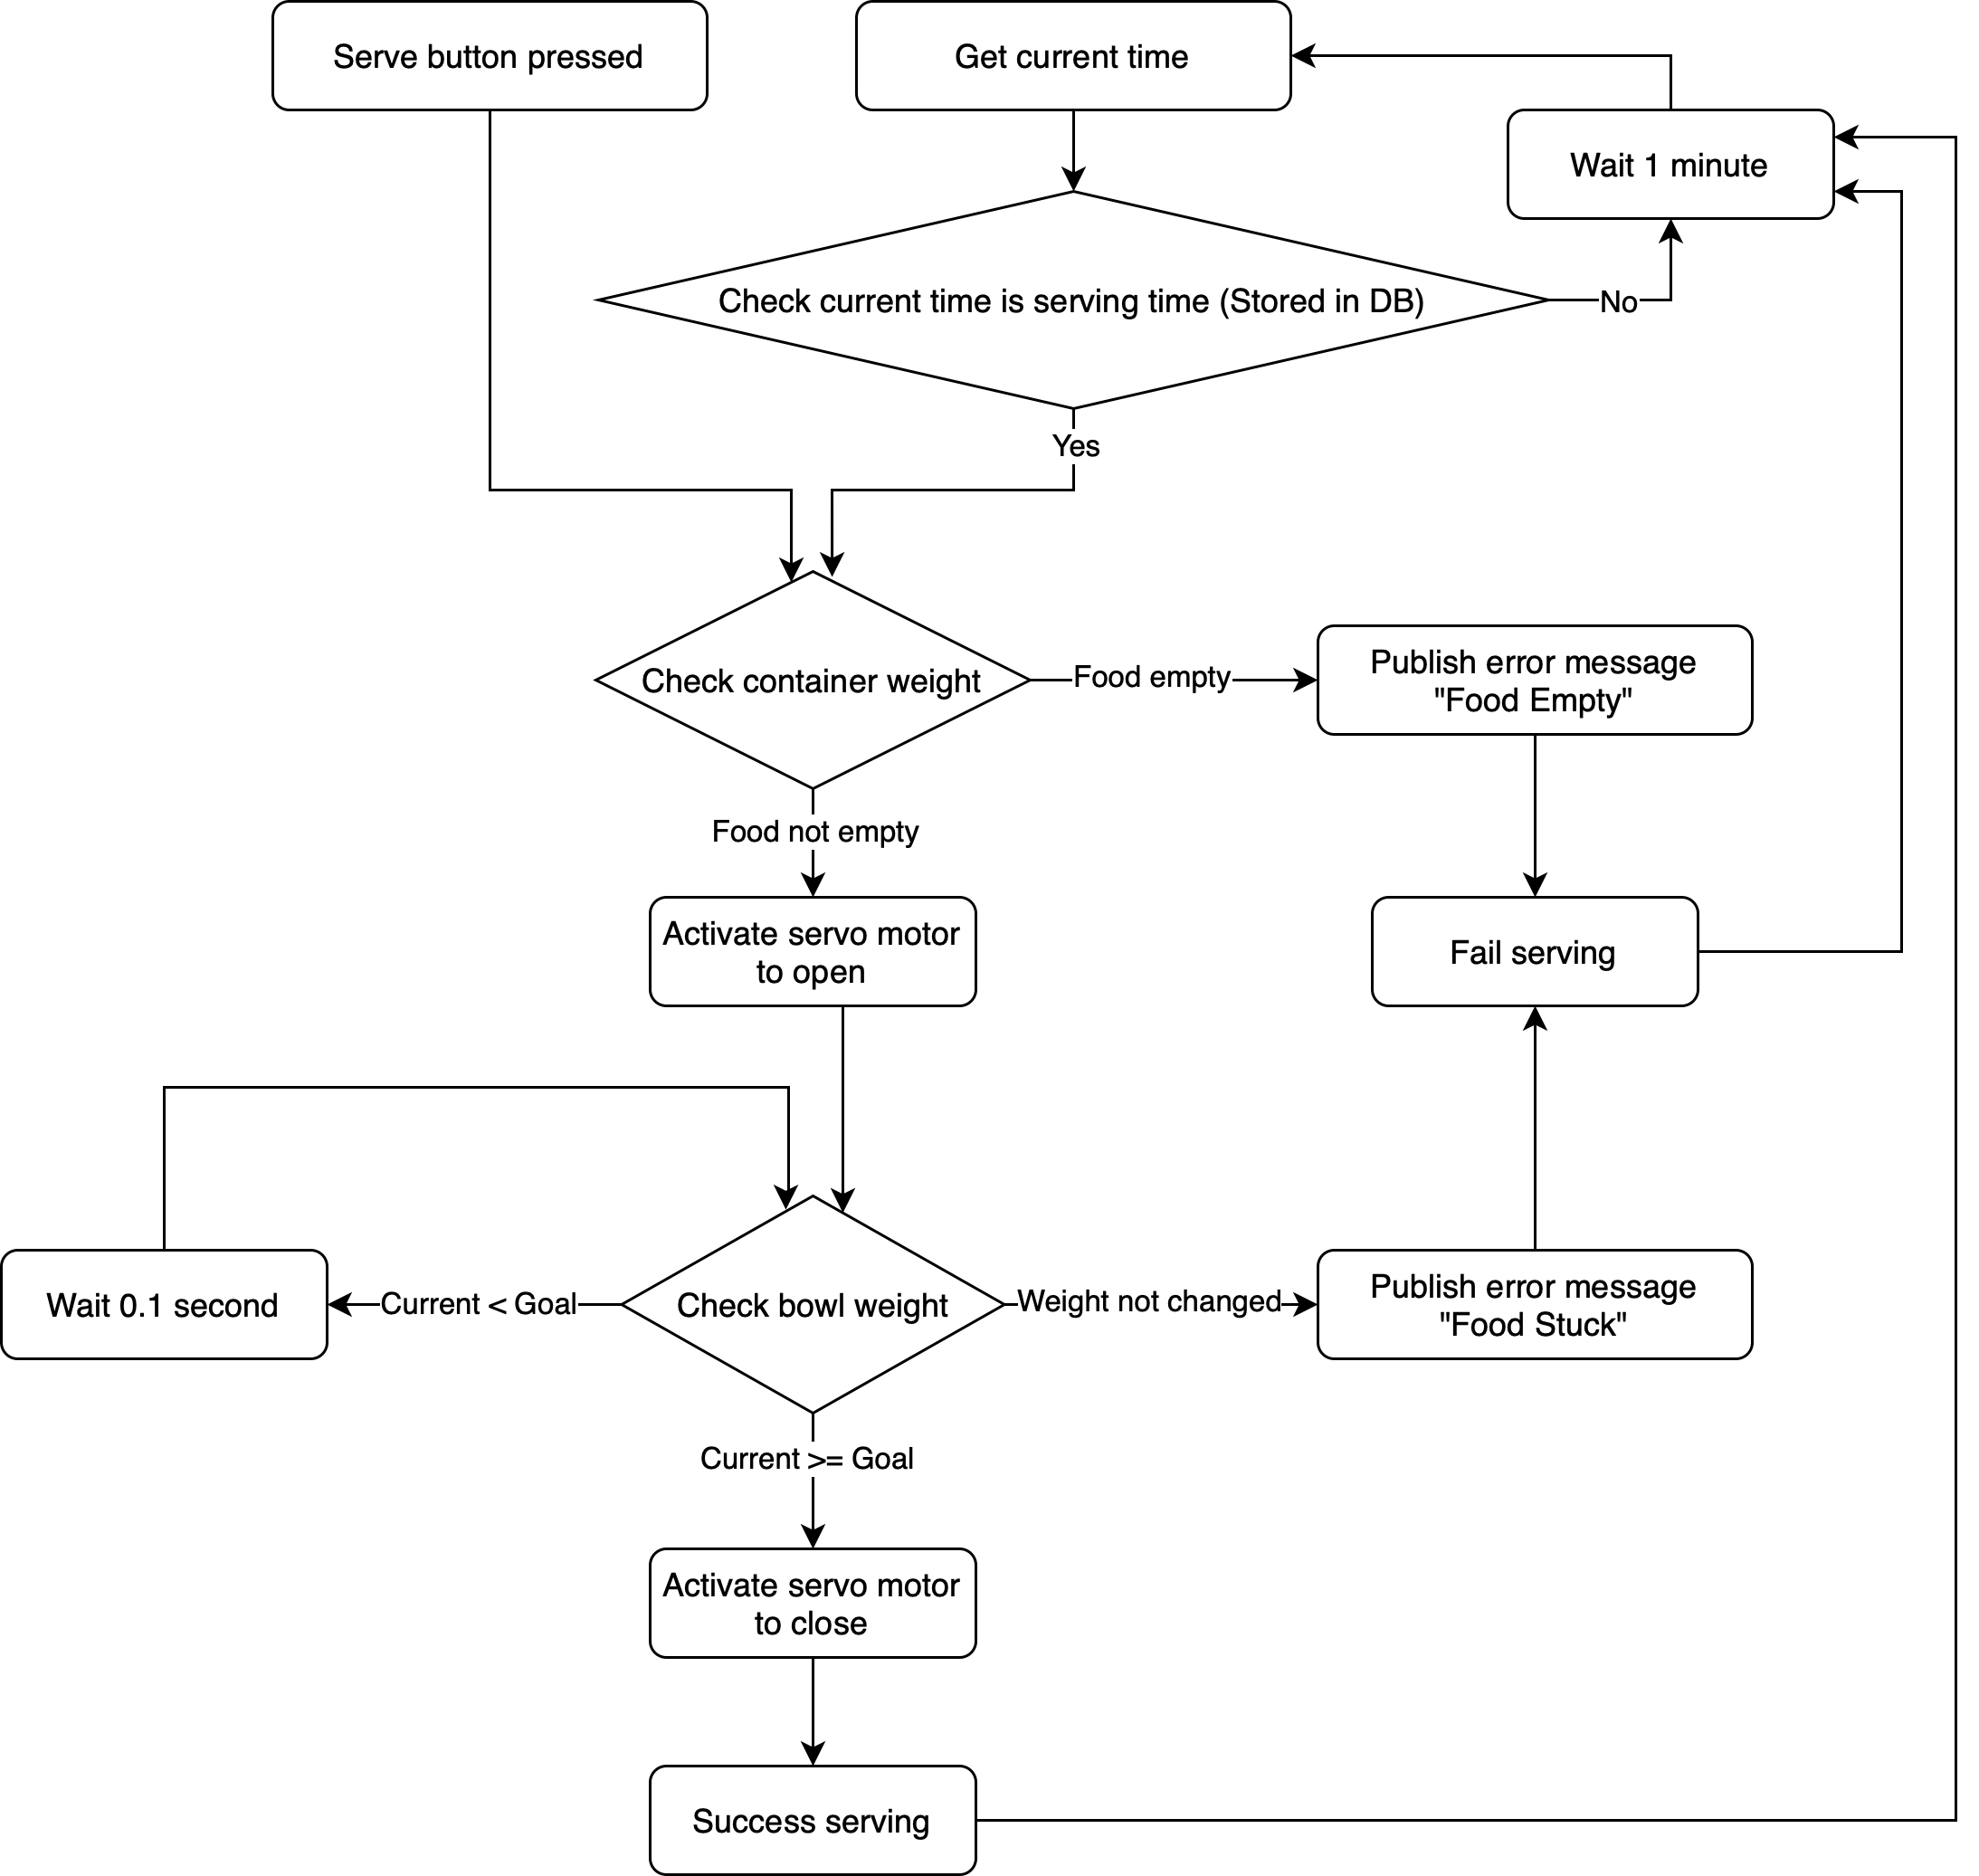
\includegraphics[width=0.5\textwidth]{FlowChart_2.png}}
\caption{Petification flow chart 2.}
\label{fig}
\end{figure}
The second flow starts when the serve button is pressed or when the previously scheduled serving time is compared with the current time.
First, measure the weight of the container, and then determine whether the container contains feed or is empty. If the container is empty, publish the error message. After that, you go back to the beginning and wait for a minute.
In the opposite case, if the container is not empty, operate the servo motor to open the container gate. From this point on, the weight of the bowl continues to be measured, and if the weight of the bowl does not change, the error that the gate is blocked will be published and flow return to wait for a minute.
If the weight of the current bowl is less than the target weight, the cycle is repeated

while waiting 0.1 seconds. When the current weight and target weight are greater or equal, the servo motor is operated to close the container gate. This is the serving success path and will return to the beginning and wait for another minute.

\hfill \break
\subsubsection{Flow3}
\begin{figure}[htbp]
\centerline{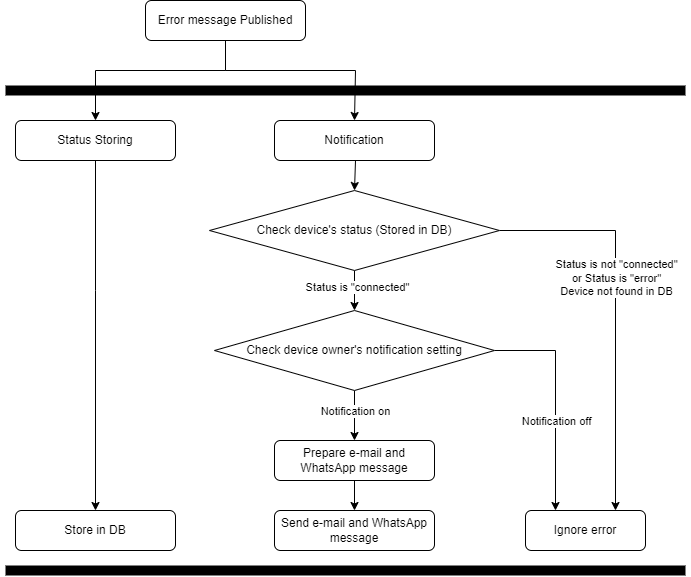
\includegraphics[width=0.5\textwidth]{FlowChart_3.png}}
\caption{Petification flow chart 3.}
\label{fig}
\end{figure}
When the device publishes an error message, two flows proceed in parallel. One is to store the current status in the DB and the other is to send an error notification.
Storing flow ends with simply storing current status in the DB, however sending error notification is not.
First, the status of the device currently stored in the DB is checked. And then, if Stauts is "connected", it moves on to the next step. If not, or if status is already error, Ignore the error message. After that, Check the notification setting of the device owner. If the notification setting is "on", prepare and send e-mail and app message. If "off", Ignore the error message. 






\section{Implementation}

\section{Experiment}
% Experiment에서는 컨테이너 높이에 따라 나오는 양이 다른지 실험 해봐야 할 듯 >> 열리는 크기는 똑같으니깐 원하는 양을 맞추면 시간을 다르게 해야함 >> 이때 열리자 마자 닫히게 하면 막히는 경우가 많았으니깐 디바이스 앞에 보강 하던 아님 최소 열리고 있어야하는 시간을 측정해서 최소 줘야하는 양을 정해야 할 듯
\section{Conclusion}

\section*{Acknowledge}
Thanks to Purdue \& IITP
\section*{References}

Please number citations consecutively within brackets \cite{b1}. The 
sentence punctuation follows the bracket \cite{b2}. Refer simply to the reference 
number, as in \cite{b3}---do not use ``Ref. \cite{b3}'' or ``reference \cite{b3}'' except at 
the beginning of a sentence: ``Reference \cite{b3} was the first $\ldots$''

Number footnotes separately in superscripts. Place the actual footnote at 
the bottom of the column in which it was cited. Do not put footnotes in the 
abstract or reference list. Use letters for table footnotes.

Unless there are six authors or more give all authors' names; do not use 
``et al.''. Papers that have not been published, even if they have been 
submitted for publication, should be cited as ``unpublished'' \cite{b4}. Papers 
that have been accepted for publication should be cited as ``in press'' \cite{b5}. 
Capitalize only the first word in a paper title, except for proper nouns and 
element symbols.

For papers published in translation journals, please give the English 
citation first, followed by the original foreign-language citation \cite{b6}.

\begin{thebibliography}{00}
\bibitem{b1} 
\bibitem{b2}
\bibitem{b3}
\bibitem{b4}
\bibitem{b5}
\bibitem{b6}
\bibitem{b7} 
\bibitem{b8}
\bibitem{b9}
\bibitem{b10}
\bibitem{b11}
\bibitem{b12}
\bibitem{b13} 
\bibitem{b14}
\bibitem{b15}
\bibitem{b16} 

% Martinviita M. (2018) "Time series database in Industrial IoT and its testing tool." Master’s Thesis, Dept. Computer Science and Engineering., University of Oulu., Pentti Kaiteran katu 1, 2018

\end{thebibliography}
\vspace{12pt}
\color{red}
IEEE conference templates contain guidance text for composing and formatting conference papers. Please ensure that all template text is removed from your conference paper prior to submission to the conference. Failure to remove the template text from your paper may result in your paper not being published.

\colorbox{red}{"this problem" undefined}

\end{document}

